%%----------------------------------------------------------
%% report_temp.tex
%% v1.0
%% 2022/10/28
%% by Carlos Rodríguez - Pardo, 2023, Universidad Carlos III de Madrid
%%----------------------------------------------------------

\documentclass{wsdcr}
\usepackage[spanish]{babel}
\usepackage{booktabs}
\usepackage{multirow}
\usepackage{markdown}
\usepackage{graphicx}

\title{%
    Predictor de bicicletas prestadas \\
    \large Análisis Avanzado de Datos - Práctica Final }
\author{Alejo Martín, Arias Filippo (NIA: 100487858)}
\date{2023}

\begin{document}

\maketitle

\section{Introducción}
Los sistemas de bicicletas compartidas se han vuelto muy populares en todo el mundo debido a su capacidad para mejorar la movilidad urbana, la salud y el medio ambiente. Estos sistemas generan grandes cantidades de datos que pueden ayudarnos a comprender mejor cómo se mueven las personas en las ciudades y qué eventos importantes ocurren en ellas. En este proyecto, vamos a utilizar un conjunto de datos de un sistema de bicicletas compartidas para construir un modelo de aprendizaje supervisado que prediga la cantidad de bicicletas alquiladas en función de diferentes factores, como la hora del día, la temperatura, la humedad y las condiciones meteorológicas.

El objetivo principal de este proyecto es mostrar cómo el aprendizaje supervisado puede ser útil para predecir la demanda de bicicletas compartidas según las condiciones ambientales y temporales, lo que podría ayudar a los operadores del sistema a mejorar la disponibilidad de bicicletas y a satisfacer mejor las necesidades de los clientes. Para lograr este objetivo, vamos a seguir un enfoque de aprendizaje supervisado, utilizando un conjunto de datos etiquetados para entrenar un modelo que pueda predecir la cantidad de bicicletas alquiladas según los diferentes factores que hemos mencionado.


\section{Descripción del Dataset}
El dataset utilizado en este proyecto es un conjunto de registros de préstamos de bicicletas compartidas en un sistema automatizado. Contiene información sobre más de 17,000 préstamos realizados cada hora durante un período de dos años, desde enero de 2011 hasta diciembre de 2012. Cada registro contiene detalles importantes, como la fecha y hora del préstamo, las condiciones climáticas, y la cantidad de bicicletas alquiladas por usuarios registrados y ocasionales.

El dataset consta de 15 columnas que proporcionan información útil sobre los patrones de préstamo de bicicletas. Las primeras columnas incluyen detalles sobre el día y la hora del préstamo, así como la temporada, el año, el mes, el día de la semana y si es un día laborable o festivo. También se registran la temperatura, la sensación térmica, la humedad y la velocidad del viento. Además, la columna "weathersit" indica las condiciones climáticas generales en la hora del préstamo. Finalmente, se incluyen tres columnas que registran el número de bicicletas alquiladas por usuarios ocasionales, usuarios registrados y el número total de bicicletas alquiladas.

\begin{itemize}
    \item \textbf{Instant}: Este es el índice de registro y no tiene un valor informativo por sí mismo.
    \item \textbf{Dteday}: Esta variable indica la fecha en que se realizó el préstamo. La fecha está en formato año-mes-día.
    \item \textbf{Hr}: Esta variable indica la hora del día en que se realizó el préstamo.
    \item \textbf{Season}: Esta variable indica la temporada en la que se realizó el préstamo. Los valores son 1 (primavera), 2 (verano), 3 (otoño) y 4 (invierno).
    \item \textbf{Year}: Esta variable indica el año en que se realizó el préstamo.
    \item \textbf{Mnth}: Esta variable indica el mes en que se realizó el préstamo.
    \item \textbf{Holiday}: Esta variable indica si el día en que se realizó el préstamo era un día festivo (1) o no (0).
    \item \textbf{Weekday}: Esta variable indica el día de la semana en que se realizó el préstamo. Los valores son 0 (domingo) a 6 (sábado).
    \item \textbf{Workingday}: Esta variable indica si el día en que se realizó el préstamo era un día laborable (1) o no (0).
    \item \textbf{Weathersit}: Esta variable indica las condiciones climáticas generales en la hora del préstamo. Los valores son 1 (despejado), 2 (nublado), 3 (lluvia ligera/nieve ligera) y 4 (lluvia intensa/nieve intensa).
    \item \textbf{Temp}: Esta variable indica la temperatura en grados Celsius en el momento del préstamo.
    \item \textbf{Atemp}: Esta variable indica la sensación térmica en grados Celsius en el momento del préstamo.
    \item \textbf{Hum}: Esta variable indica la humedad relativa en el momento del préstamo.
    \item \textbf{Windspeed}: Esta variable indica la velocidad del viento en km/h en el momento del préstamo.
    \item \textbf{Casual}: Esta variable indica el número de bicicletas alquiladas por usuarios ocasionales en la hora del préstamo.
    \item \textbf{Registered}: Esta variable indica el número de bicicletas alquiladas por usuarios registrados en la hora del préstamo.
    \item \textbf{Count}: Esta variable indica el número total de bicicletas alquiladas en la hora del préstamo (es decir, la suma de los valores de las variables Casual y Registered).
\end{itemize}

\section{Descripción del problema}
En este proyecto, nuestro objetivo es predecir el número de bicicletas que se alquilarán en una hora determinada utilizando un modelo de aprendizaje supervisado. Para lograr esto, vamos a considerar varias variables que podrían influir en la cantidad de bicicletas alquiladas.

Una de las variables más importantes es la hora del día, ya que se espera que la cantidad de bicicletas alquiladas varíe a lo largo del día debido a los patrones de movilidad de las personas. Es posible que haya más alquileres de bicicletas durante las horas pico de la mañana y la tarde, cuando la gente se dirige al trabajo o regresa a casa.

Otra variable importante es el clima. Las condiciones climáticas pueden tener un gran impacto en la cantidad de bicicletas alquiladas. Es posible que haya menos alquileres de bicicletas en días lluviosos o fríos, mientras que en días soleados y cálidos se pueden alquilar más bicicletas.

Además, las variables de temperatura, humedad y velocidad del viento también pueden tener un efecto en la cantidad de bicicletas alquiladas. Es posible que las personas estén menos dispuestas a alquilar bicicletas en días extremadamente calurosos o húmedos.

Finalmente, es importante tener en cuenta las variables relacionadas con los usuarios, como la cantidad de usuarios registrados y ocasionales. Es posible que los patrones de alquiler difieran según el tipo de usuario y que los usuarios registrados alquilen bicicletas con más frecuencia que los usuarios ocasionales.

\section{Análisis de los datos}

\begin{verbatim}
    |            |       cnt |
    |:-----------|----------:|
    | instant    |  0.278379 |
    | weekday    |  0.0268999|
    | workingday |  0.0302844|
    | weathersit | -0.142426 |
    | atemp      |  0.400929 |
    | windspeed  |  0.0932338|
    | hum        | -0.322911 |
    | casual     |  0.694564 |
    | registered |  0.972151 |
    | cnt        |  1        |
\end{verbatim}

La tabla muestra la correlación entre la variable dependiente "cnt" (número total de bicicletas alquiladas) y las diferentes variables independientes en el conjunto de datos.

Se puede observar que la variable más fuertemente correlacionada con "cnt" es "registered" (correlación positiva de 0.972), que representa el número de usuarios registrados que alquilan bicicletas. La variable "casual" (correlación positiva de 0.695) también tiene una fuerte correlación con "cnt", lo que indica que los usuarios no registrados también tienen un impacto significativo en el número total de bicicletas alquiladas.

Además, se puede observar una correlación positiva moderada entre "cnt" y "atemp" (0.401), que representa la temperatura ajustada. Esto sugiere que los usuarios tienen más probabilidades de alquilar bicicletas en días con temperaturas más cálidas.

Por otro lado, se puede observar una correlación negativa moderada entre "cnt" y "hum" (-0.323), que representa la humedad. Esto sugiere que los usuarios tienen menos probabilidades de alquilar bicicletas en días más húmedos.

Finalmente, "weathersit" (condiciones meteorológicas) y "windspeed" (velocidad del viento) tienen una correlación débil y negativa con "cnt", lo que sugiere que estos factores no tienen un impacto significativo en el número total de bicicletas alquiladas.

\begin{figure}[h]
    \centering
    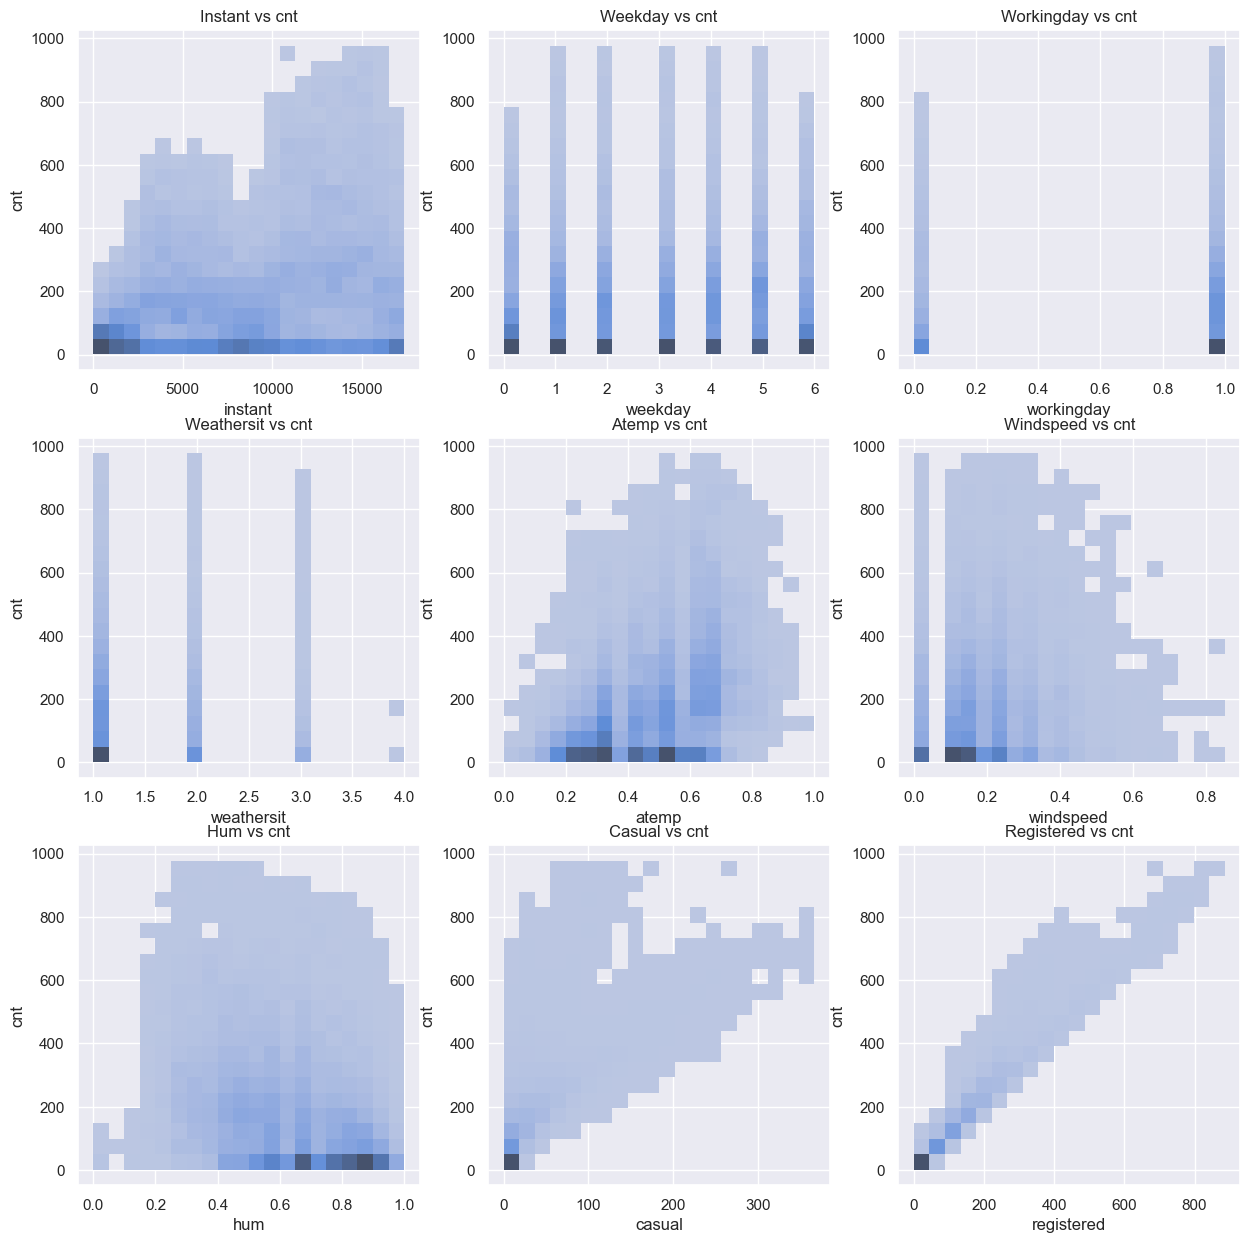
\includegraphics[width=0.4\textwidth]{charts/histograms.png}
    \caption{Histogramas}
    \label{fig:histograms}
\end{figure}

\begin{figure}[h]
    \centering
    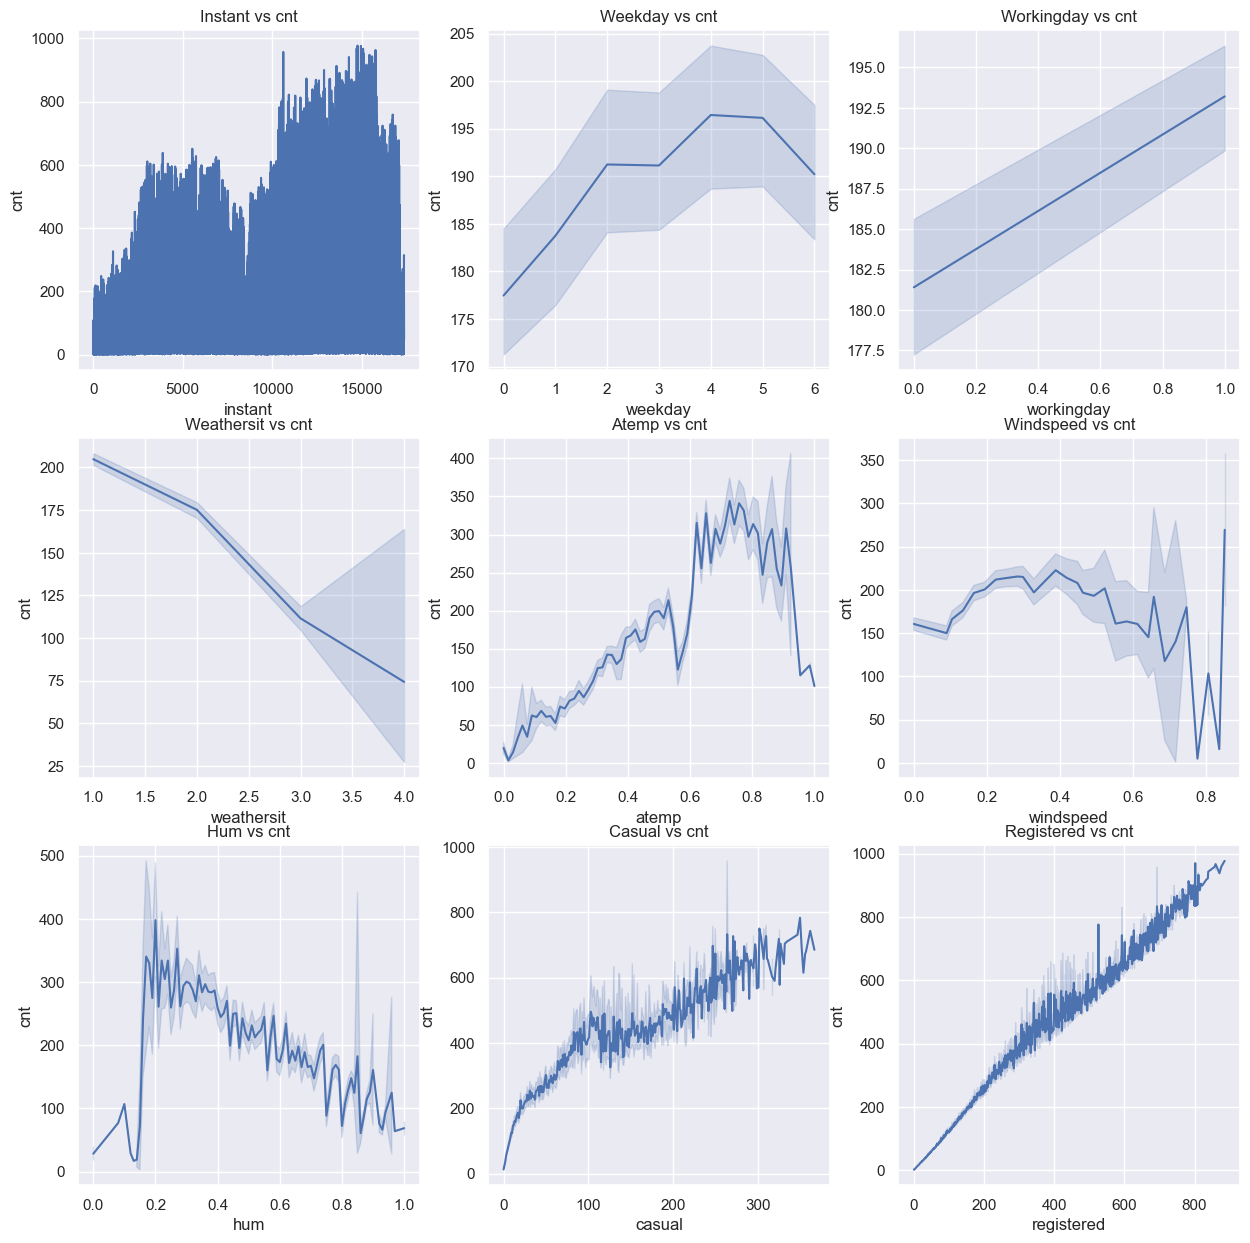
\includegraphics[width=0.4\textwidth]{charts/line-charts.png}
    \caption{Gráfico de líneas}
    \label{fig:linecharts}
\end{figure}

\begin{figure}[h]
    \centering
    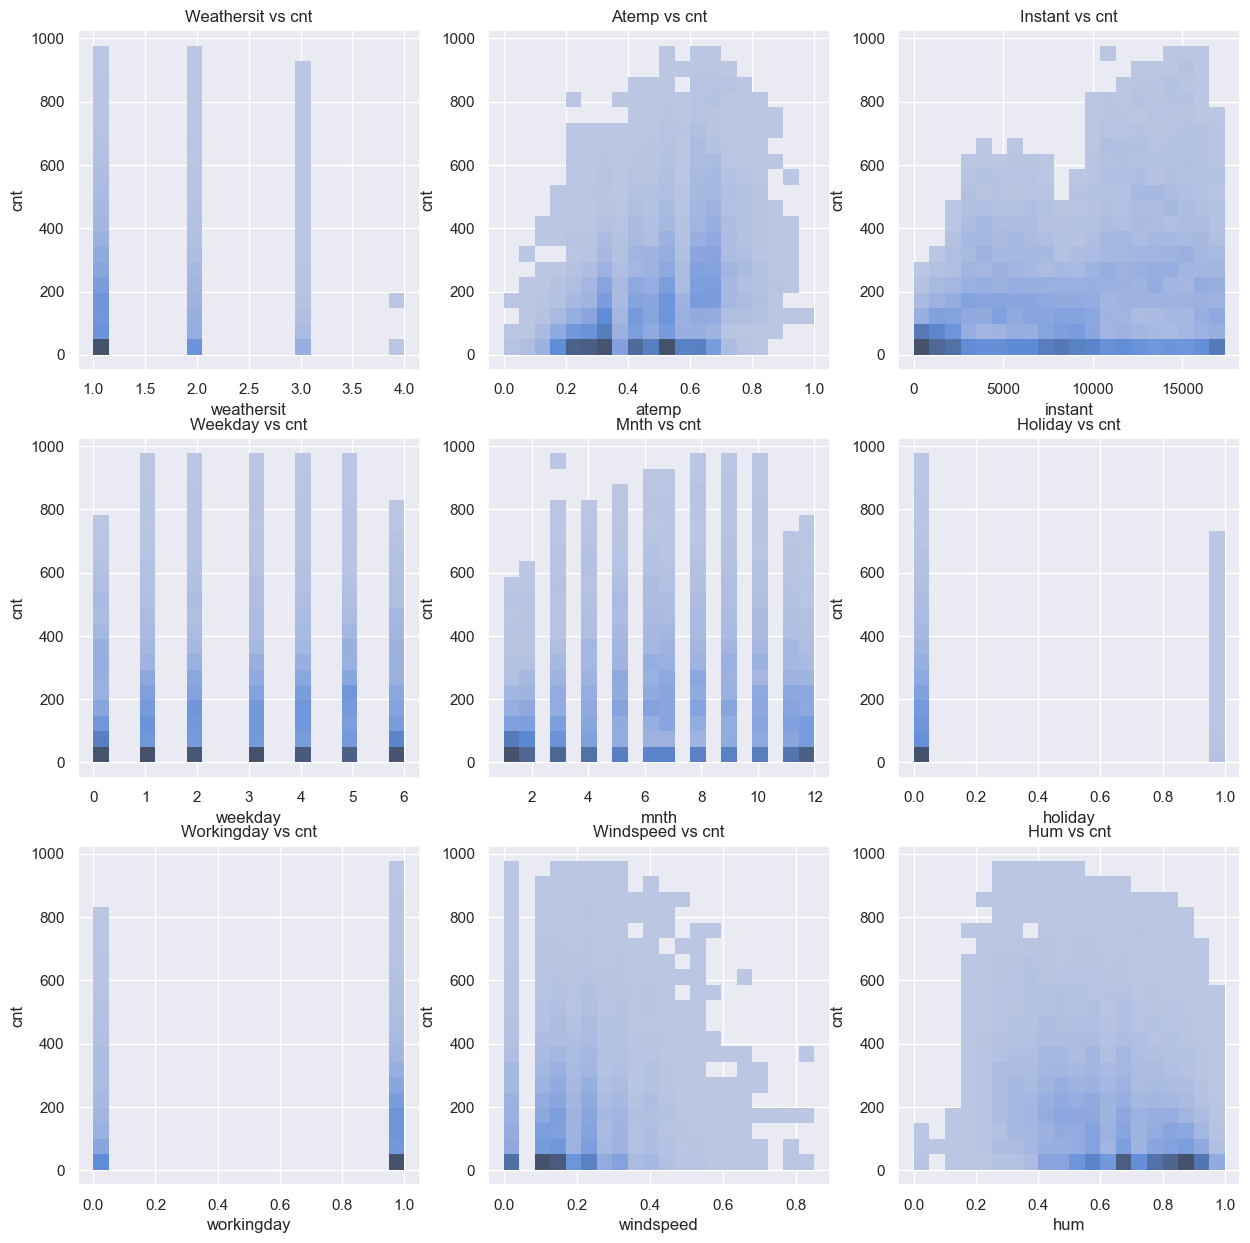
\includegraphics[width=0.4\textwidth]{charts/correlational-matrix.png}
    \caption{Matriz correlacional}
    \label{fig:correlationmatrix}
\end{figure}

Para obtener los histogramas, utilizamos la función hist de la librería matplotlib, que nos permite visualizar la distribución de cada variable. Para obtener los gráficos de líneas correlacional, utilizamos la función plot de la misma librería, pasando como parámetros las variables a graficar y la variable cnt. Finalmente, para obtener la matriz correlacional, utilizamos la función heatmap de la librería seaborn.

Estos gráficos nos permiten visualizar las relaciones entre las variables y la variable cnt. Los histogramas nos muestran la distribución de cada variable, mientras que los gráficos de líneas correlacional nos permiten ver la relación entre cada variable y cnt. La matriz correlacional nos muestra la relación entre todas las variables.

De esta forma, podemos relacionar las conclusiones obtenidas en la última tabla con los gráficos obtenidos. Por ejemplo, la correlación positiva entre la variable atemp y cnt se refleja en el gráfico de líneas correlacional correspondiente, donde podemos ver una tendencia positiva entre ambas variables. Del mismo modo, la correlación negativa entre hum y cnt se refleja en el gráfico correspondiente, donde podemos ver una tendencia negativa entre ambas variables. Los histogramas nos muestran la distribución de cada variable y nos permiten ver si hay valores atípicos o si los datos siguen una distribución normal. La matriz correlacional nos muestra todas las correlaciones entre las variables, lo que nos permite tener una visión general de la relación entre todas las variables en conjunto.

\section{Método}

\subsection{Aprendizaje supervisado}
En primer lugar, dividiremos nuestros datos en un conjunto de entrenamiento y un conjunto de prueba. A continuación, aplicaremos diferentes técnicas de regresión, como la regresión lineal o la regresión polinómica, para modelar la relación entre las variables independientes (día de la semana, hora del día, temperatura, etc.) y la variable dependiente (número de bicicletas alquiladas).

Una vez que hayamos entrenado nuestro modelo de regresión, evaluaremos su rendimiento utilizando diferentes métricas, como el error cuadrático medio o el coeficiente de determinación. Si nuestro modelo tiene un buen rendimiento en el conjunto de prueba, lo utilizaremos para hacer predicciones sobre la demanda futura de bicicletas.

\subsection{Aprendizaje no supervisado}
Se utilizaran ténicas de clustering y reducción de dimensionalidad.
En el caso del clustering, agruparíamos los datos en diferentes grupos o clústeres según su similitud, lo que nos permitiría identificar patrones y características comunes en los datos. Esto podría ser útil para segmentar la demanda de bicicletas y detectar posibles oportunidades de negocio.

Por otro lado, la reducción de dimensionalidad nos permitiría reducir el número de variables o características en nuestros datos sin perder información importante. Esto podría ser útil si tenemos un gran número de variables y queremos simplificar nuestro modelo de regresión sin perder precisión en nuestras predicciones.

\section{Resultados}

\subsection{Limitaciones}

\section{Conclusiones y Trabajo Futuro}







\appendices
\section{}
Appendix uno va aquí.

% you can choose not to have a title for an appendix
% if you want by leaving the argument blank
\section{}
Appendix dos va aquí.


% use section* for acknowledgment
\bibliographystyle{IEEEtran}
%% you can change the style into any other styles available, I personally love IEEEtran.
\bibliography{citations}
%% to generate references, input the name of your .bib file and cite anywhere in the document.

\end{document}
